\documentclass[a4paper, 11pt, oneside]{book}
\usepackage{/home/nicolas/Documents/Enseignement/Prepa/bpep/fichiers_utiles/preambule}

\newcommand{\dsNB}{1}
\makeatletter
\renewcommand{\@chapapp}{Kh\^olles MPSI3 -- semaine \dsNB}
\makeatother

\toggletrue{corrige}  % décommenter pour passer en mode corrigé

\begin{document}

\resetQ
\newpage

\chapter{Sujet 1\siCorrige{\!\!-- corrigé}}
\section{Question de cours}

Donner et démontrer la relation de conjugaison d'un miroir plan.

\section{Grenouille intelligente}

\QR{Pour se cacher des prédateurs, une grenouille s'est accrochée sous un
    nénuphar qui flotte sur l'étang. La grenouille a une hauteur $h$ et le
    nénuphar un rayon $R$ et une épaisseur très faible.

    Quel doit être le rayon minimal $R_0$ du nénuphar pour que les pieds de la
    grenouille ne soient pas visibles par un prédateur situé en-dehors de
l'eau?}{
\begin{tcbraster}[raster columns=7, raster equal height=rows]
    \begin{NCdefi}[raster multicolumn=4]{Données}
        Pour une hauteur de grenouille fixée, il y a une taille de
        nénuphar permettant à tous les rayons partant de la grenouille de ne
        pas traverser le dioptre.\smallbreak
        \begin{center}
            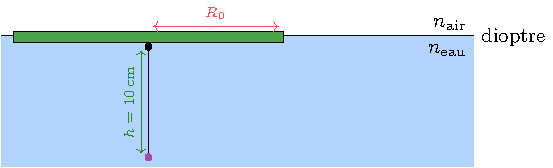
\includegraphics{../../figures/ch2-2-1}   
        \end{center}
    \end{NCdefi}
    \begin{tcolorbox}[blankest, raster multicolumn=3, space to=\myspace]
        \begin{tcbraster}[raster columns=1]
            \begin{NCprop}{But à atteindre}
                Origine physique de ce phénomène et traduction mathématique.
            \end{NCprop}    
            \begin{NCrapp}{Outils du cours}
                Loi de Snell-Descartes :
                \[ n_1\sin i_1 = n_2\sin i_2\]
                et \underline{angle limite} de réfraction, tel que :
                \[ n_1\sin i_\ell = n_2\sin \ang{90;;} = n_2\]
                qui indique que pour $n_1 > n_2$, il y a un angle d'incidence à
                partir duquel il n'y a pas de rayon réfracté (les rayons
                réfractés font un angle de 90° avec la normale et sont donc
                parallèles au dioptre).
            \end{NCrapp}
        \end{tcbraster}
    \end{tcolorbox}
\end{tcbraster}

\begin{NCexem}[breakable]{Application}
    Pour que les pieds de la grenouille ne soient pas visibles par un prédateur
    situé en-dehors de l'eau, c'est-à-dire au-dessus du dioptre, il faut
    simplement qu'il n'y ait pas de rayon partant de ses pieds et qui puissent
    sortir de l'eau : il faut que tous les rayons avec un angle d'incidence plus
    faible que cet angle limite soient bloqués par le nénuphar. C'est possible
    puisqu'on est dans une situation où le rayon passe dans un milieu
    \textbf{moins réfringent}, i.e. $n_2 < n_1$. En effet, dans cette situation
    il y a une inclinaison du rayon incident qui implique que le rayon émergent
    est parallèle à la surface, et tous les rayons au-delà de cet angle limite
    sont tous réfléchis. Un beau, grand schéma avec toutes les données reportées
    dessus mène naturellement à l'utilisation de formules trigonométriques de
    4\ieme.
    \begin{center}
        \vspace*{-2.5cm}
        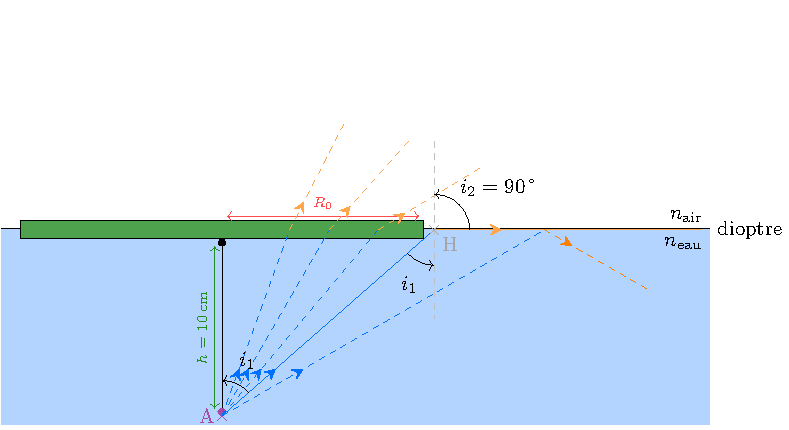
\includegraphics{../../figures/ch2-2-2}
    \end{center}
    On voit ici qu'une simple fonction $\tan$ permet d'exprimer $R_0$ :
    \begin{empheq}[box=\fbox]{align}\label{eq:tan}
        \tan i_1 = \frac{R_0}{h}
    \end{empheq}
    Seulement on n'a pas encore la valeur de $i_1$. Or, on a déterminé que pour
    fonctionner l'astuce de la grenouille est d'avoir $i_1 = i_\ell$, et d'après
    le cours :
    \begin{empheq}{align}
        n\eau\sin i_\ell       & = n\air\\
        \Leftrightarrow i_\ell & = \asin \frac{n\air}{n\eau}\label{eq:ilim}
    \end{empheq}
    On peut donc écrire, avec \ref{eq:tan} et \ref{eq:ilim} :
    \begin{empheq}[box=\fbox]{equation}
        R_0 = h\times\tan\left(\asin \frac{n\air}{n\eau}\right)
        \quad \text{avec}
        \left\{
            \begin{array}{rcl}
                h & = & \SI{10.0}{cm}\\
                n_\mathrm{air} & = & \num{1.00}\\
                n_\mathrm{eau} & = & \num{1.33}
            \end{array}
        \right.
    \end{empheq}
    et finalement,
    \begin{empheq}[box=\fbox]{equation}
        R_0 = \SI{11.4}{cm}
    \end{empheq}
\end{NCexem}
}

\resetQ
\subimport{/home/nicolas/Documents/Enseignement/Prepa/bpep/exercices/Colle/prisme_Dove/}{sujet.tex}

\resetQ
\newpage

\chapter{Sujet 2\siCorrige{\!\!-- corrigé}}
\section{Question de cours}

Définir un rayon lumineux et énoncer les propriétés liées à leur propagation.

\subimport{/home/nicolas/Documents/Enseignement/Prepa/bpep/exercices/Colle/refractometreAbbe/}{sujet.tex}

\resetQ
\newpage

\chapter{Sujet 3\siCorrige{\!\!-- corrigé}}
\section{Question de cours}

Définir la notion de stigmatisme et d'aplanétisme, les conditions de Gauss et
leur conséquence.

\subimport{/home/nicolas/Documents/Enseignement/Prepa/bpep/exercices/Colle/Capteur_de_niveau_d_eau/}{sujet.tex}

\resetQ
\newpage

\chapter{Sujet 4\siCorrige{\!\!-- corrigé}}
\section{Question de cours}

Qu'est-ce qu'un système optique centré ? Comment sont définis les points objet
et image ? Comment sont définis le caractère réel et virtuel point un point et
un objet ? Accompagner chaque réponse d'un schéma.

\section{Prisme rectangle}

\QR{On utilise un prisme de verre d'indice $n=\num{1.5}$. Sa section principale
    est un triangle $ABC$ rectangle en $A$ tel que l'angle en $B$ soit égal à
    \ang{70;;}. Un rayon lumineux dans le plan $ABC$ rencontre le prisme en $I$
    sur le côté $AB$ perpendiculairement à $AB$. Sachant que le rayon incident
    est dans l'air, étudier la marche de la lumière jusqu'à la sortie du
prisme.}{
\begin{tcbraster}[raster columns=3, raster equal height=rows]
    \begin{NCdefi}[raster multicolumn=2]{Schéma}
        \begin{center}
            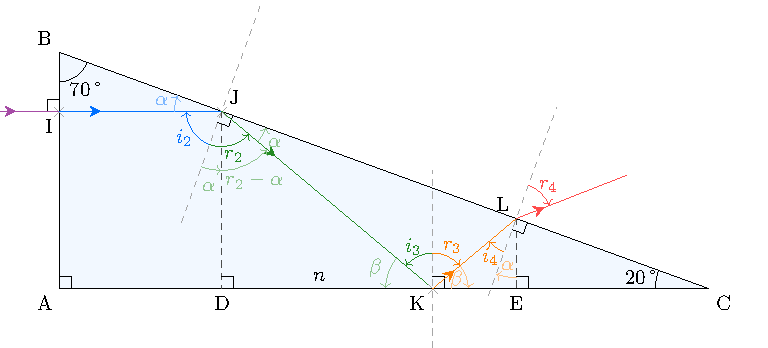
\includegraphics[scale=0.94]{../../figures/ch2-9}
            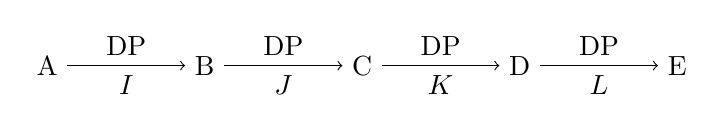
\begin{tikzpicture}[]
                \node[] (A) at (0,0) {A};
                \node[] (B) at (2,0) {B};
                \node[] (C) at (4,0) {C};
                \node[] (D) at (6,0) {D};
                \node[] (E) at (8,0) {E};
                \draw[->] (A) -- (B)
                    node [midway, above] {DP}
                    node [midway, below] {$I$};
                \draw[->] (B) -- (C)
                    node [midway, above] {DP}
                    node [midway, below] {$J$};
                \draw[->] (C) -- (D)
                    node [midway, above] {DP}
                    node [midway, below] {$K$};
                \draw[->] (D) -- (E)
                    node [midway, above] {DP}
                    node [midway, below] {$L$};
            \end{tikzpicture}
        \end{center}
    \end{NCdefi}
    \begin{tcolorbox}[blankest, raster multicolumn=1, space to=\myspace]
        \begin{tcbraster}[raster columns=1]
            \begin{NCprop}[]{Résultat attendu}
                On cherche à suivre le chemin du rayon indiqué dans l'énoncé. Il
                faut pour cela savoir ce qui peut arriver au rayon. Dans le cas
                du passage par un dioptre plan, il peut y avoir traversée du
                dioptre avec Snell-Descartes, ou réflexion dans le cas $n_2 <
                n_1$.
            \end{NCprop}
            \begin{NCrapp}{Outils du cours}
                Loi de Snell-Descartes :
                \[ n_1\sin i = n_2\sin r\]
                et pour $n_2 < n_1$, $i_\ell$ :
                \[ n_1\sin i_\ell = n_2\sin \ang{90;;} = n_2\]
                tel que $i_1 > i_\ell$ est réfléchi.
            \end{NCrapp}
        \end{tcbraster}
    \end{tcolorbox}
\end{tcbraster}
\begin{NCexem}[sidebyside]{Application}
    Ici, l'angle limite de réflexion à l'intérieur du prisme est : \[i_\ell =
    \arcsin \frac{1}{n} = \boxed{ \ang{41.8;;}}\]
    \begin{description}
        \item[I] : $\boxed{i_1 = \ang{0;;}}$ donc
            $\boxed{r_1 = \ang{0;;}}$ ;
        \item[J] : Ici, on doit voir que $\alpha = \ang{20;;}$ puisque
            dans le triangle BIJ, la somme des angles doit valoir $\ang{180;;}$
            et qu'on a un angle droit + un angle de \ang{70;;}.
            On en déduit que $\boxed{i_2 = \ang{70;;}}$ également, car
            $i_2 + \alpha = \ang{90;;}$.\smallbreak
            Comme \underline{$i_2 > i_\ell$}, le rayon ne traverse pas mais est
            réfléchi, soit $\boxed{r_2 = \ang{70;;}}$.
    \end{description}
    \tcblower
    \begin{description}
        \item[K] : Pour trouver l'angle en K, on peut par exemple chercher
            l'angle $\beta$ : en construisant le triangle rectangle JDK, on
            trouve que l'angle au sommet est $r_2 - \alpha = \ang{50;;}$ ;
            avec l'angle droit en D, $\beta = \ang{40;;}$, et $\boxed{i_3
            = \ang{50;;} > i_\ell}$ donc rayon réfléchi $\boxed{r_3 =
        \ang{50;;}}$.
        \item[L] : De même qu'en J, tracer LEC indique que $i_4 + \alpha + \beta
            = \ang{90;;}$, soit $\boxed{i_4 = \ang{30;;} < i_\ell}$
            : on applique donc Snell-Descartes ici, et on obtient
            \[\boxed{r_4} = \arcsin (n\times \sin i_4) =
            \boxed{\ang{48.6;;}}\]
    \end{description}
\end{NCexem}

}

\resetQ
\newpage

\chapter{Sujet 5\siCorrige{\!\!-- corrigé}}
\section{Question de cours}

Énoncer les conditions de réflexion totale \textit{avec un schéma}, donner et
démontrer la valeur de l'angle limite $i_{\rm lim}$ en fonction de $n_2$ et
$n_1$.

\subimport{/home/nicolas/Documents/Enseignement/Prepa/bpep/exercices/Colle/angle_brewster/}{sujet.tex}
\resetQ
\subimport{/home/nicolas/Documents/Enseignement/Prepa/bpep/exercices/Colle/vitre_pare_brise/}{sujet.tex}

\end{document}
